\documentclass[11pt]{article}

% Change "review" to "final" to generate the final (sometimes called camera-ready) version.
% Change to "preprint" to generate a non-anonymous version with page numbers.
\usepackage[review]{acl}

% Standard package includes
\usepackage{times}
\usepackage{latexsym}

% For proper rendering and hyphenation of words containing Latin characters (including in bib files)
\usepackage[T1]{fontenc}
% For Vietnamese characters
% \usepackage[T5]{fontenc}
% See https://www.latex-project.org/help/documentation/encguide.pdf for other character sets

% This assumes your files are encoded as UTF8
\usepackage[utf8]{inputenc}

% This is not strictly necessary, and may be commented out,
% but it will improve the layout of the manuscript,
% and will typically save some space.
\usepackage{microtype}

% This is also not strictly necessary, and may be commented out.
% However, it will improve the aesthetics of text in
% the typewriter font.
\usepackage{inconsolata}

%Including images in your LaTeX document requires adding
%additional package(s)
\usepackage{graphicx}

% Additional packages for tables and math
\usepackage{booktabs}
\usepackage{amsmath}

\title{Political Bias and Temporal Dynamics in Large Language Models}

\author{Ran Lu \\
  Université Paris-Saclay \\
  \texttt{ran.lu@universite-paris-saclay.fr} \\\And
  Hasti Hosseinpour \\
  Université Paris-Saclay \\
  \texttt{hasti.hosseinpour@universite-paris-saclay.fr} \\\And
  Abderrahmane Moujar \\
  Université Paris-Saclay \\
  \texttt{abderrahmane.moujar@universite-paris-saclay.fr} \\\And
  Oloruntobi Olutola \\
  Université Paris-Saclay \\
  \texttt{oloruntobi.olutola@universite-paris-saclay.fr}}

\begin{document}
\maketitle

\begin{abstract}
LLMs exhibit systematic political biases, but most work treats bias as static. We study political bias as a temporal phenomenon using Prediction Inconsistency (IC) and sentiment label distributions. We evaluate ChatGPT (gpt-3.5-turbo through gpt-4o) and Llama~3.2 (Base and Instruct) on target-oriented sentiment classification. IC jumps from $\approx$0 (gpt-3.5-turbo) to $\approx$0.67 (gpt-4) and plateaus at $\approx$0.61 for later GPT-4 variants; Llama IC is lower (0.005--0.178) and instruction tuning strongly reduces it for the 1B model. Label distributions shift from all-positive (gpt-3.5-turbo) to positive/UNKNOWN mixes (GPT-4) and vary by size and alignment for Llama.
\end{abstract}

\section{Introduction}

LLMs are increasingly used to access and interpret political information; their latent political orientations have real consequences \citep{santurkar2023,buyl2026,hartmann2023,bang2024}. Most prior work evaluates bias at a single point in time, yet model families evolve rapidly in training data, safety, and alignment \citep{touvron2023,dubey2024}. We study political bias over time using Prediction Inconsistency (IC) \citep{elbouanani2025} and sentiment label distributions on two families: OpenAI ChatGPT and Meta Llama. We ask: (1) How does IC change across model generations? (2) How does alignment (Base vs.\ Instruct) affect IC and label distribution? Our contributions: a temporal view of political bias, longitudinal IC and label-distribution results for ChatGPT and Llama, and evidence that alignment effects are size- and family-dependent.

\section{Related Work}

Prior work measures political bias via ideological mapping \citep{santurkar2023,hartmann2023}, stance vs.\ framing \citep{bang2024}, and target-oriented sentiment \citep{wang2025,chen2024}. Temporal drift in LLM behavior and bias is documented \citep{zhu2024,buyl2026}; LLaMA evolution illustrates changes in safety and alignment \citep{touvron2023,dubey2024}. Mitigation and alignment can alter political nuance \citep{banko2025,bonaldi2024}. We extend \citet{elbouanani2025} to a temporal, multi-family setting.

\section{Methodology}

We follow \citet{elbouanani2025}: 250 political entities, 60 sentence templates (positive/neutral/negative), entity substitution, and target-oriented sentiment classification (TSC) with labels $\{\text{positive}, \text{neutral}, \text{negative}\}$. Political bias is Prediction Inconsistency (IC): entropy of predicted labels across entities per template, averaged over templates. For template $s$, $P(l|s) = |\{e \in E : \text{pred}(s,e)=l\}|/|E|$; $H(s) = -\sum_l P(l|s)\log P(l|s)$; $\text{IC} = \frac{1}{m}\sum_i H(s_i)$. IC=0 means perfectly consistent (unbiased). We use 9-shot prompting, temperature=0, and identical prompt sets across versions. Models: ChatGPT (gpt-3.5-turbo, gpt-4, gpt-4-turbo, gpt-4o-mini, gpt-4o); Llama~3.2 Base (1b, 3b) and Instruct (1b, 3b, vision 11b).

\section{Results}

\textbf{ChatGPT (Figure~\ref{fig:results}, left).} IC is near zero for gpt-3.5-turbo, jumps to $\approx$0.67 for gpt-4, and plateaus at $\approx$0.61 for gpt-4-turbo, gpt-4o-mini, and gpt-4o (mean 0.501). Label distribution: gpt-3.5-turbo 100\% positive; gpt-4 $\approx$60\% positive, 40\% UNKNOWN; gpt-4-turbo / gpt-4o-mini / gpt-4o $\approx$30\% positive, 70\% UNKNOWN. No neutral or negative in this eval.

\textbf{Llama (Figure~\ref{fig:results}, right).} Base: IC 1b $\approx$0.178, 3b $\approx$0.118. Instruct: 1b $\approx$0.028, 3b $\approx$0.120, vision 11b $\approx$0.005. Instruction tuning strongly reduces IC for 1b; 3b is similar in Base and Instruct; 11b has lowest IC. Label distribution: Base 1b/3b skew negative; Instruct 1b $\approx$97--98\% negative; Instruct 3b and 11b show more positive/neutral (e.g., 11b $\approx$32\% positive, 30\% neutral, 34\% negative).

\begin{figure*}[t]
  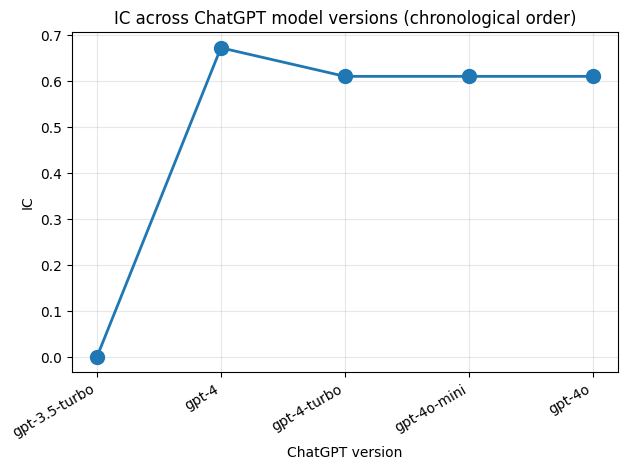
\includegraphics[width=0.48\textwidth]{figures/chatgpt_ic_chronological.png}
  \hfill
  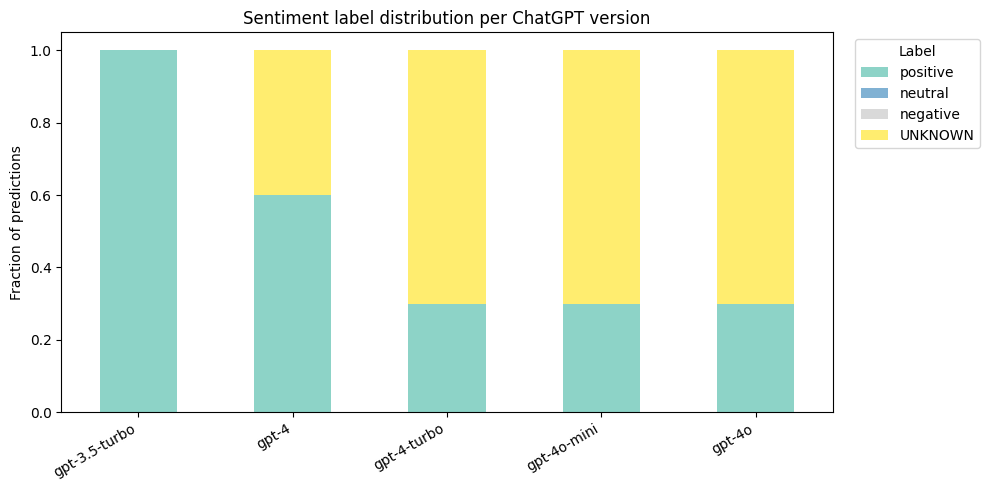
\includegraphics[width=0.48\textwidth]{figures/llama_ic_base_instruct.png}
  \caption{Left: IC across ChatGPT versions (chronological). Right: IC for Llama~3.2 Base vs.\ Instruct.}
  \label{fig:results}
\end{figure*}

\section{Discussion \& Conclusion}

ChatGPT shows a sharp IC increase from gpt-3.5-turbo to gpt-4 and a plateau for later gpt-4 variants; the shift to large UNKNOWN shares may reflect refusal/hedging while still yielding high inconsistency. For Llama, instruction tuning reduces IC for 1B but not 3B; the 11B vision model has minimal IC. Alignment effects on both IC and label distribution are size- and family-dependent. Cross-family, ChatGPT has higher IC (0.61--0.67) than Llama (0.005--0.178) and different label patterns (positive/UNKNOWN vs.\ negative/neutral). Limitations: two families and fixed versions; IC does not capture all bias dimensions; UNKNOWN share complicates interpretation. Future work: more families, time horizons, and bias metrics.

\section*{Acknowledgments}
We thank Prof. Adrian Popescu (Fairness in AI, Université Paris-Saclay) and the TEMPO-BIAS project.

% Bibliography entries for the entire Anthology, followed by custom entries
\bibliography{custom}

\end{document}
